\section{Results and Discussion}
System-level simulation was performed with representative AI inference workloads.

\begin{itemize}
  \item \textbf{Standby Power}: $>$30\% reduction by migrating cold data to FeRAM-backed tier.
  \item \textbf{Resume Latency}: reduced to $\mu$s–ms range, enabling instant resume across power cycles.
  \item \textbf{Endurance}: $10^{12}$ writes/year fits within FeRAM capability for checkpoint traffic.
\end{itemize}

% ===== Fig.2: Access time vs Retention (TikZ + PGFPlots) =====
\begin{figure}[!t]
\centering
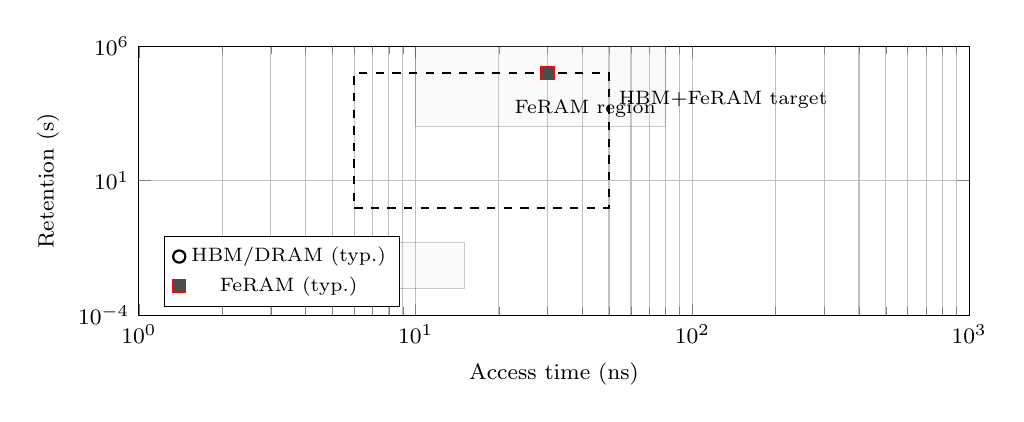
\begin{tikzpicture}
\begin{loglogaxis}[
  width=\linewidth,
  height=5.0cm,
  xlabel={Access time (ns)},
  ylabel={Retention (s)},
  xmin=1e0, xmax=1e3,
  ymin=1e-4, ymax=1e6, % 指定レンジ
  grid=both,
  label style={font=\footnotesize},
  tick label style={font=\footnotesize},
  legend style={font=\scriptsize, at={(0.03,0.03)}, anchor=south west},
  clip=false
]
% points
\addplot+[only marks, mark=*, mark size=2.2pt, mark options={fill=white,draw=black,thick}]
  coordinates {(5, 1e-2)}; \addlegendentry{HBM/DRAM (typ.)}
\addplot+[only marks, mark=square*, mark size=2.4pt, mark options={fill=black!70}]
  coordinates {(30, 1e5)}; \addlegendentry{FeRAM (typ.)}
% regions
\addplot [draw=black, fill=black!10, opacity=0.20]
  coordinates {(2,1e-3) (15,1e-3) (15,5e-2) (2,5e-2)} -- cycle;
\node[anchor=north west, font=\scriptsize] at (axis cs:2,5e-2){DRAM region};
\addplot [draw=black, fill=black!10, opacity=0.18]
  coordinates {(10,1e3) (80,1e3) (80,1e6) (10,1e6)} -- cycle;
\node[anchor=south east, font=\scriptsize] at (axis cs:80,1e3){FeRAM region};
% hybrid target box (dashed)
\addplot [draw=black, dashed, thick]
  coordinates {(6,1e0) (50,1e0) (50,1e5) (6,1e5)} -- cycle;
\node[anchor=west, font=\scriptsize] at (axis cs:50,1e4){HBM+FeRAM target};
\end{loglogaxis}
\end{tikzpicture}
\caption{Access time vs retention. Hybrid HBM+FeRAM expands the usable design space toward fast \& persistent operation.}
\label{fig:retention_map}
\end{figure}
